% vim: spell:spelllang=en:
\documentclass[12pt, oneside]{article}
\usepackage[a4paper, left=2.5cm, right=2.5cm, top=2.5cm, bottom=2.5cm]{geometry}

\usepackage[utf8]{inputenc} % Use unicode
\usepackage[T1]{fontenc}
\usepackage[english]{babel} % Names in spanish

%% Bibliography:
%\usepackage{comment}
%\usepackage[
    %backend=biber,
    %style=numeric,
%]{biblatex}
%\DeclareNameAlias{default}{last-first}

%\usepackage{csquotes}       % For bibliography quotations
%\DeclareQuoteAlias{spanish}{catalan}

%\addbibresource{biblio.bib}
%% see:
%% https://www.sharelatex.com/learn/Bibliography_management_in_LaTeX#The_bibliography_file

%\usepackage{datetime} % Customize date
%% \monthyeardate\today gives the date without the day
%\newdateformat{monthyeardate}{%
    %\monthname[\THEMONTH], \THEYEAR}

% For cross references
\usepackage[colorlinks = true]{hyperref}
\usepackage[catalan]{varioref}
%\usepackage{cleveref}
%hyperref configuration so that it doesn't contrast so much colorlinks,
\hypersetup{
   linkcolor={black},
   citecolor={black},
   %linkcolor={red!50!black},
   %citecolor={blue!50!black},
   urlcolor={blue!80!black}
}

\usepackage{xcolor}     % color

\usepackage{mathtools}  % amsmath + more
\usepackage{amsthm}     % Theorem enviroment
\usepackage{amssymb}    % More symbols
\usepackage{amstext}    % Text inside mathenv

\usepackage{relsize}    % Bigger math with mathlarger{___}
\usepackage{nicefrac}   % nice fractions in one line

\usepackage[export]{adjustbox}  % Adjust table size
\usepackage{float}              % Force tables and images position (H and H!)
\usepackage{wrapfig}            % Wrap images like in HTML

\usepackage{tabularx, colortbl, booktabs}    % Better tables
\usepackage{longtable}                      % Multiple page table

% Split cell in lines and more formating options inside table
\usepackage{array, multirow, multicol, makecell}

%\usepackage{subcaption}                     % Subfigures
%\usepackage[framemethod=tikz]{mdframed}     % Custom frames

%\usepackage[bottom]{footmisc} % Footnotes at bottom of page

%\usepackage[alsoload=hep]{siunitx}          % SI units and uncertainties
%\sisetup{locale = FR}                       % Commas and so on for spanish
%\sisetup{separate-uncertainty=true}
%\sisetup{
  %per-mode=fraction,
  %fraction-function=\nicefrac
%}

%\usepackage{tikz}
%%\usetikzlibrary{arrows}
%%\usetikzlibrary{scopes}
%\usetikzlibrary{babel}

%\usepackage{listings}       % For code blocks

%% Custom code highlight
%\definecolor{codegreen}{rgb}{0,0.6,0}
%\definecolor{codegray}{rgb}{0.5,0.5,0.5}
%\definecolor{codepurple}{rgb}{0.58,0,0.82}
%\definecolor{backcolour}{rgb}{0.95,0.95,0.92}
%\definecolor{lightblue}{RGB}{135,206,250}

%\lstdefinestyle{mystyle}{ backgroundcolor=\color{backcolour},
    %commentstyle=\color{codegreen}, keywordstyle=\color{blue},
    %numberstyle=\tiny\color{codegray}, stringstyle=\color{red},
    %identifierstyle=\color{black}, basicstyle=\footnotesize,
    %%breakatwhitespace=false,
    %breaklines=true,
    %%captionpos=b,                    keepspaces=true,
    %numbers=left,                    numbersep=5pt,
    %showspaces=false,
    %%showstringspaces=false, showtabs=false,
    %tabsize=4
%}
%\lstset{style=mystyle}

\newcommand{\whitepage}{
    \clearpage\thispagestyle{empty}\addtocounter{page}{-1} \newpage \clearpage
}

% Add command before appendix session for page numbering: A-1
%\newcommand{\appendixpagenumbering}{
    %\break
    %\pagenumbering{arabic}
    %\renewcommand{\thepage}{\thesection-\arabic{page}}
%}

%% Custom Math operators (functions not in italic in math mode):
%\DeclareMathOperator{\arcsec}{arcsec}
%\DeclareMathOperator{\arccot}{arccot}
%\DeclareMathOperator{\arccsc}{arccsc}
%\DeclareMathOperator{\cis}{cis}


\usepackage{caption}
\usepackage{subcaption}
\usepackage{graphicx}
\usepackage{enumitem}
\usepackage{lipsum}

\usepackage{siunitx}
\usepackage{hyphenat}

\usepackage{xcolor}

\usepackage{minted}
\setminted{
frame=lines,
framesep=2mm,
baselinestretch=1.2,
breaklines,
%bgcolor=LightGray,
fontsize=\footnotesize,
linenos
}

\renewcommand\theadfont{\bfseries}

\title{
    PAR Laboratory Assignment\\
    Lab 2: Brief tutorial on OpenMP programming model
}

\author{
    par2109:
    Aleix Boné,
    Alex Herrero
}

\date{
    Spring 2019-20
}

\begin{document}

\thispagestyle{empty}
\clearpage
\setcounter{page}{-1}

\begin{titlepage}
{
    \centering
    \null
    \vfill
    {\Huge \bfseries PAR Laboratory Assignment\par}
    \vspace{3em}
    {\Large {\scshape Lab 2:} Brief tutorial on OpenMP programming model\par}
    \vfill
\begin{center}
\end{center}
    \vspace{3cm}

    \vfill
    {\raggedleft \Large
        Aleix Boné\\
        Alex Herrero\\
        {\bfseries\ttfamily par2109}\\
        \vspace{4em}
        2020-03-27
        \par}
}
\end{titlepage}

% \pagenumbering{arabic} 
% vale perf, lo envias tu? okidoki
% seems good to me %perf
\section{OpenMP questionnaire}%
\label{sec:OpenMP questionnaire}

%When answering to the questions in this questionnaire, please DO NOT simply answer with yes, no or a number; try to minimally justify all your answers and if necessary include any code fragment you need to support your answer.  Sometimes you may need to execute several times in order to see the effect of data races in the parallel execution.

\begin{enumerate}[label=\textbf{\Alph*)}]
    \item \textbf{Parallel regions} \\
    \textbf{1.hello.c:}
    \begin{enumerate}[label=\arabic*.]
        \item 24 since the boada server has 24 cores so \emph{OpenMP} defaults to 24 threads.
        \item If we specify the number of threads that \emph{OpenMP} can use with the environment variable \texttt{OMP\_NUM\_THREADS=4} we will only
        see 4 \texttt{"Hello World!"} messages.
    \end{enumerate}
    \textbf{2.hello.c:}
    \begin{enumerate}[label=\arabic*.]
        \item Since the variable \texttt{id} is shared by default, there are times when the number displayed are not correct.
        (There are pairs of Hello that share the same number or numbers that don't appear). To fix this we have to add
        the clause \texttt{private(id)} to our directive.
        \item The lines not always are printed in the same order and sometimes they appear inter-mixed since the execution is parallel and some threads might end before the others.
    \end{enumerate}
    \textbf{3.howmany.c:}
    \begin{enumerate}[label=\arabic*.]
        \item There are printed 20 \texttt{"Hello world ..."} lines.
        The first Hello world is printed 8 times since there are 8 threads defined with the environment
        variable \texttt{OMP\_NUM\_THREADS}. The second Hello world runs 2 times for the first iteration of
        the loop where we set the number of threads with the function \texttt{omp\_set\_num\_threads(i)} and
        3 for the second iteration. The third parallel runs 4 times since we specify 4 threads on the
        pragma. The last parallel region prints 3 times since the call \texttt{omp\_set\_num\_threads(3)} 
        set the threads to 3. This makes a total of:  8 + 2 + 3 + 4 + 3 = 20.
        \item Inside the parallel region it returns the number of threads executed in parallel, outside it
        returns 1 since there is only on thread.
    \end{enumerate}
    \textbf{4.datasharing.c:}
    \begin{enumerate}[label=\arabic*.]
        \item With the attribute \texttt{shared} we got that \texttt{x} is usually 120 but sometimes it gets lower values because we have a race condition since += reads the value and then writes to it.
        With \texttt{private} attribute \texttt{x} is always 5 since it's private each thread has its own value of x
        that is independent from the \texttt{x} of the main thread, so \texttt{x} is never updated.
        With \texttt{firstprivate} it's also 5 since its the same as \texttt{private} but with the only difference that the variable \texttt{x} of
        each thread is initialized with the value on the main thread and with \texttt{private} it's not.
        Finally, with \texttt{reduction} it's always 125. Which is $5 + 1 + 2 + \dots + 16$.
    \end{enumerate}
    \pagebreak
    \item \textbf{Loop parallelism} \\
    \textbf{1.schedule.c:}
        \begin{itemize}
            \item[] \texttt{static}: The threads get assigned iterations is chunks of 3 $(12/4=3)$ in order: the first thread gets iterations 0 to 2,
            the seconds gets 3 to 5 an so on.
            \item[] \texttt{static, 2}: The threads get assigned iterations in chunks of 2 in order: the first thread gets iterations 0 and 1,
            the second 2 and 3 and so on. Since there are not enough threads to run all the 12 iterations in parallel in chunks of 2,
            the first and second thread also get assigned the iterations 8,9 and 10,11 respectively.
            \item[] \texttt{dynamic, 2}: The threads get assigned iterations in chunks of 2 without any other. The order will depend on
            which thread is available to process the chunks as they are needed.
            \item[] \texttt{guided, 2}: With guided scheduling the threads get assigned iterations initially in chunks of 2 but the size
            of the chunks increases throughout the loop.
        \end{itemize}
    \textbf{2.nowait.c:}
    \begin{enumerate}[label=\arabic*.]
        \item Any thread can get any of the iterations because the scheduling is dynamic so there is no order guaranteed, the only thing we can know is that the first thread will be assigned to the first iteration of the loop.
        
        % The possible sequences of \texttt{printf} are all the : % esto no lo tengo claro, pork si es dynamic i no se espera puede que pase qualquier combinacion, no? PUES TIENE PINTA QUE ES LO TUYO, ASÍ QUE DECIMOS ESO Y PONEMOS UN EJEMPLO (ya lo hago yo). HAGO ESTO y luego la tabla si e sisi
        % ok yo quitaria la mayoria de mierdas esta de quote pot tampoco aportan mucho
        % gracias! estaba en blanco jajaja
        % yo despues de escribir toda la mierda de antes ya estoy en modo bullshit total 
        % te rellen aqui qualquier chorrada en un plis plas
        % jajajaj me sirve, tu bullshit no es tan bullshit como crees 
        % the good kind of bullshit jajajaja
        
        % se pueden borrar las quotes
        %\begin{quote}
        %    \texttt{Loop 1: thread (0) gets iteration 0 \\
        %    Loop 1: thread (1) gets iteration 1 \\
        %    Loop 2: thread (2) gets iteration 2 \\
        %    Loop 2: thread (3) gets iteration 3}
        %\end{quote}
        %also:
        %\begin{quote}
        %    \texttt{Loop 1: thread (0) gets iteration 0 \\
        %    Loop 1: thread (1) gets iteration 1 \\
        %    Loop 2: thread (3) gets iteration 2 \\
        %    Loop 2: thread (2) gets iteration 3}
        %\end{quote}
        %and:
        %\begin{quote}
        %    \texttt{Loop 1: thread (0) gets iteration 0 \\
        %    Loop 1: thread (3) gets iteration 1 \\
        %    Loop 2: thread (1) gets iteration 2 \\
        %    Loop 2: thread (2) gets iteration 3}
        %\end{quote}
        \item If we remove the \texttt{nowait}, the iterations must finish before the loop continues, so Loop 1 will always output before Loop 2.
        %  Pues nose, borraamos los ejemplos o como lo explico? YO SI BORRARIA LOS EJEMPLOS CON LO QUE DICES YA QUEDA CLARO CREO YO.
        %In this case the only possible sequences are:
        %\begin{quote}
        %    \texttt{Loop 1: thread (0) gets iteration 0 \\
        %    Loop 1: thread (1) gets iteration 1 \\
        %    Loop 2: thread (2) gets iteration 2 \\
        %    Loop 2: thread (3) gets iteration 3}
        %\end{quote}
        %and:
        %\begin{quote}
        %    \texttt{Loop 1: thread (1) gets iteration 0 \\
        %    Loop 1: thread (0) gets iteration 1 \\
        %    Loop 2: thread (3) gets iteration 2 \\
        %    Loop 2: thread (2) gets iteration 3}
        %\end{quote}
        
        \item If we change \texttt{dynamic} to \texttt{static}, the order of assignment of the threads will be the same,
        even with the \texttt{nowait} clause. And only 2 threads will be used since the for loops have 2 iterations. The
        output will always be:
        \begin{quote}
            \texttt{Loop 1: thread (0) gets iteration 0 \\
            Loop 1: thread (1) gets iteration 1 \\
            Loop 2: thread (0) gets iteration 2 \\
            Loop 2: thread (1) gets iteration 3}
        \end{quote}
        
    \end{enumerate}
    \textbf{3.collapse.c:}
    \begin{enumerate}[label=\arabic*.]
        \item As shown in the next table, the thread 0 execute the first four iterations, the thread 1 executes the next three consecutive iterations and so on until the thread number 7 executes the three last iterations of the loop.
        %\begin{table}[H]%se puede borrar perfectamente
        %\centering
        %\begin{tabular}{cl}
        %\toprule
        %    Thread & Iterations \\
        %\midrule
        %    0   & $(0\, 0) \rightarrow (0\, 3)$ \\
        %    1   & $(0\, 4) \rightarrow (1\, 1)$ \\
        %    2   & $(1\, 2) \rightarrow (1\, 4)$ \\
        %    3   & $(2\, 0) \rightarrow (2\, 2)$ \\
        %    4   & $(2\, 3) \rightarrow (3\, 0)$ \\
        %    5   & $(3\, 1) \rightarrow (3\, 3)$ \\
        %    6   & $(3\, 4) \rightarrow (4\, 1)$ \\
        %    7   & $(4\, 2) \rightarrow (4\, 4)$ \\
        %\bottomrule
        %\end{tabular}
        %\label{tab:3.collapse-thread-iterations}
        %\end{table}
        \item Without \texttt{collapse} it's not correct, not all indices of the matrix are shown, because \texttt{j} is declared
        before the pragma and therefore it's shared among the threads which. We should add the \texttt{private(j)} clause so that the different 
        threads don't interfere with one another.

    \end{enumerate}
    \pagebreak
    \item \textbf{Synchronization} \\
    \textbf{1.datarace.c:}
    \begin{enumerate}[label=\arabic*.]
        \item We tried 100 executions of the program with: 
        
        \texttt{for i in \{1..100\}; do ./1.datarace; done | grep Sorry -c}
        
        and we got 100 wrong 0, 
        correct. The program almost always will produce the wrong output. This happens because there is a data race when reading and updating the value
        of the shared variable \texttt{x}.
        \item To make it correct we must make sure that the reads and writes to \texttt{x} of the threads are properly synchronized. We can do that
        by replacing the clause \texttt{shared(x)} by \texttt{reduction(+: x)}. Another option is to add the directive \texttt{\#pragma omp atomic} or 
        \texttt{\#pragma omp critical} before the instruction \texttt{x++}.
    \end{enumerate}
    \textbf{2.barrier.c:}
    \begin{enumerate}[label=\arabic*.]
        \item We can predict that all threads will output first their going to sleep messages and since the time it takes to display the message is
        much less than the time the threads sleep and we have enough threads they fill most certainly output the message of waking up after all the threads
        have printed their sleep messages, although there is no guarantee. Once they \emph{all} threads print their wake up messages, the barrier will
        unlock and they will display the \emph{We are all awake!} message, this time there is a barrier so its guaranteed that no thread will
        reach the \emph{We are all awake!} message before all threads have reached the barrier.
        
        It seems there is no specific order in which the threads exit the barrier although in our experiments, most of the time, the last thread that
        outputs the \emph{wakes up and enters barrier} message is the first to exit it.
    \end{enumerate}
    \textbf{3.ordered.c:}
    \begin{enumerate}[label=\arabic*.]
        \item The order of the \emph{Outside} messages is non-deterministic since it depends on the dynamic scheduling of the threads.
        In the other hand, the order of the \emph{Inside} messages is always the same relative to themselves and they follow the order
        that the loop would have if executed sequentially (0, 1, 2, \dots, N).
        \item If we modify the clause \texttt{schedule} to include a chunk size of 2 like so: \texttt{schedule( dynamic, 2)} the tasks
        will get assigned 2 consecutive iteration of the loop.
    \end{enumerate}
    \pagebreak
    \item \textbf{Tasks} \\
    \textbf{1.single.c:}
    \begin{enumerate}[label=\arabic*.]
        \item Since we have the \texttt{nowait} clause on our \texttt{single} directive, all four threads are assigned the single clauses
        of the loop without waiting for them to finish. They appear to be executed in burst since although we have \texttt{nowait}, we only
        have 4 threads so they all run 4 tasks, sleep for 1 second, they finish roughly at the same time and get assigned to the 4 next iterations.
    \end{enumerate}
    \textbf{2.fibtasks.c:}
    \begin{enumerate}[label=\arabic*.]
        \item Because there is no \mintinline{cpp}{#pragma omp parallel} directive and therefore no threads are created.
        \item To execute it correctly in parallel we have to add \mintinline{cpp}{#pragma omp parallel}
         and \mintinline{cpp}{#pragma omp single} and the clause \texttt{firstprivate(p)} As shown below:

    \begin{minted}[firstnumber=66]{cpp}
#pragma omp parallel
#pragma omp single
while (p != NULL) {
    printf("Thread %d creating task that will compute %d\n", omp_get_thread_num(), p->data);
    #pragma omp task firstprivate(p)
        processwork(p);
    p = p->next;
}
    \end{minted}
     
    \end{enumerate}
    \textbf{3.synchtasks.c:}
    \begin{enumerate}[label=\arabic*.]
        \item As we can see in Figure~\ref{graph:3synchtasks} \texttt{foo1} and \texttt{foo2} must be done before \texttt{foo4} and at the same time \texttt{foo4} before \texttt{foo5}.
        \begin{figure}[H]
        \centering
        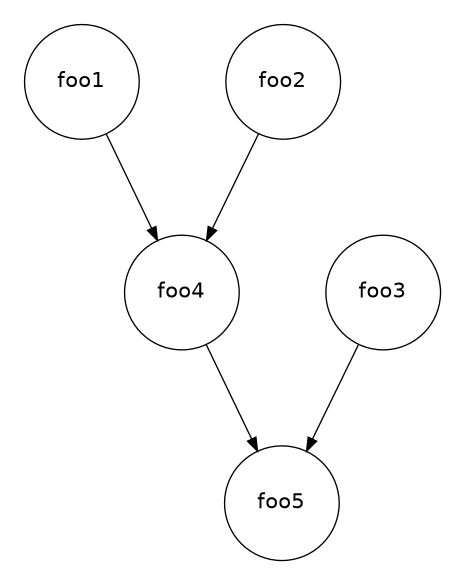
\includegraphics[width=0.35\textwidth]{3.synchtasks_taskDependence.png}
        \caption{Task dependence graph of \texttt{3.synchtasks.c}}
        \label{graph:3synchtasks}
        \end{figure}
        \item To make the program execute properly using only \texttt{taskwait}, we have to put a one
        \texttt{taskwait} before every task that has a dependency, in this case we put them before
        \texttt{foo4} and \texttt{foo5}:
        
        \begin{minted}[firstnumber=41]{cpp}
int main(int argc, char *argv[]) {
    #pragma omp parallel
    #pragma omp single
    {
    	printf("Creating task foo1\n");
    	//#pragma omp task depend(out:a)
        #pragma omp task
    	foo1();
    	printf("Creating task foo2\n");
    	//#pragma omp task depend(out:b)
        #pragma omp task
    	foo2();
    	printf("Creating task foo3\n");
    	//#pragma omp task depend(out:c)
        #pragma omp task
    	foo3();
    	printf("Creating task foo4\n");
    	//#pragma omp task depend(in: a, b) depend(out:d)
        #pragma omp taskwait
        #pragma omp task
    	foo4();
    	printf("Creating task foo5\n");
    	//#pragma omp task depend(in: c, d)
        #pragma omp taskwait
        #pragma omp task
    	foo5();
    }
    return 0;
}
        \end{minted}
    \end{enumerate}
    \textbf{4.taskloop.c:}
    \begin{enumerate}[label=\arabic*.]
        \item With \texttt{grainsize} each task gets 6 iterations.
        With \texttt{num\_tasks} each task gets 3 iterations, this is due to the fact that there are 4 threads (which is less
        than 5) and 12 iterations, so each task gets $\frac{12}{3} = 4$ iterations of the loop.
        \item If we add the \texttt{nogroup} clause, the taskloop does not create an implicit \texttt{taskgroup} and therefore the program
        does not wait for the execution of the first loop to finish before moving to the next step.
    \end{enumerate}
\end{enumerate}

\section{Observing overheads}
\label{sec:observing_overheads}
% Please explain in this section of your deliverable the main results obtained and your conclusions in terms of overheads for parallel,task and the
% different synchronisation mechanisms.  Include any tables/plots that support your conclusions.

\subsection{Synchronisation overheads}

%Take a look at the four different versions and make sure you understand them.  For example, how many synchronisation operations (critical or atomic) are executed in each version?
% esto no se verlo y xD 

%atmoc i critical hacen el mismo numero de syncros 1 antes 1 una despues % solo 2? y que tienen de distinto?
%creo k sumlocal hace lo mismo que reduction en el fondo Lo que no veo es pork hay tanta differencia% ya pero en teoria hacen lo mismo, no? mmmh
%no hay mucha dif entre estos dos justamente no? yokse

\begin{table}[H]
\centering
\begin{tabular}{lrrr}
\toprule
    & 1 thread & 4 threads & 8 threads \\
\midrule
    \texttt{Critical}    & 4.358014s     & 37.993402s    & 35.054946s    \\
    \texttt{Atomic}      & 1.820260s     & 6.537028s     & 6.638720s     \\
    \texttt{Reduction}   & 1.838303s     & 0.475096s     & 0.251802s     \\
    \texttt{Sumlocal}    & 1.844493s     & 0.482096s     & 0.249314s     \\
\midrule
    Sequential version   & 1.793754s     &               &               \\
\bottomrule
\end{tabular}

\caption{Execution times of 100.000.000 iterations} 
\label{tab:Execution_time}
\end{table}

%If executed with only 1 thread and 100.000.000 iterations, do you observe any major overhead in the execution time caused by the use of the different synchronisation mechanisms? You can compare with the baseline execution time of the sequential version in pisequential.c. = 1.793754101s

%As shown in table~\ref{tab:Execution_time} when executing with only one thread and 100.000.000 iterations we notice that there is a major overhead with the \texttt{critical} synchronisation mechanism as it's more than double the time of sequential version in \texttt{pisequential.c}.
%This is because each access to \emph{sum} in the \texttt{critical} version is protected ensuring exclusive access to it so that it can only be accessed
%by one thread at a time which introduces synchronization for every iteration of the loop.

\begin{itemize}
\item[--] \texttt{critical}: The \texttt{critical} region protects access to the sum ensuring exclusive access to it. This means
that it can only be accessed by one thread at a time and that we have to perform a synchronization for every iteration of the loop.
This introduces massive overhead while giving no real benefit since most of the code is affected by this region an thus is not
parallel. In the table we can appreciate how much more time it takes (even in the 1 thread version) compared to the sequential version
and the rest of the parallel versions.
\item[--] \texttt{atomic}: This is similar to the \texttt{critical} region since it protects the same variable, the main difference
is that the synchronization is performed at the memory access at a hardware level which allows for a smaller sequential region to
synchronize. We can see in the table that is much better than its \texttt{critical} counterpart but it still introduces too much
overhead when having to synchronize multiple threads.
\item[--] \texttt{reduction}: In this version the synchronization only occurs once all the tasks generated by the for loop finish
and then their values for \emph{sum} which where independent for each thread are added together. This allows the parallel execution
of all the tasks generated by the \texttt{for} loop since there is no dependence between the iterations. This is reflected on the
results shown on the table in which we achieve an Speedup of 7.12 with 8 threads.
\item[--] \texttt{sumlocal}: This version of the code performs the same operations that \texttt{reduction}, but instead of
using the built-in directive of \emph{OpenMP} the code is modified to perform the reduction manually. The results obtained are
very similar to the \texttt{reduction}, this shows that both versions are equivalent.
\end{itemize}

%i que ponemos?
%la idea es meter lo k ya tenemos en la bullet list. para que quede todo similar y se lea fluido. 
% pero claro es raro.
% igual primero una aclaracion sobre al ejecucion en 1 thread i luego hablas de multithreads en la lista.This me gusta
% puedes utilizar lo de abajo ~/ref{this} lol jeje

%con que digas quantas operaciones de syncro haces en cada cosa ya queda bien explicado diria. ves a donde estoy yo XD

%If executed with 4 and 8 threads and the same number of iterations,  do the 4 programs benefit from the use of several processors in the same way?  Can you guess the reason for this behaviour.

%We can also observe that when executed with 4 and 8 threads and the same number of iterations the \texttt{critical} and the \texttt{atomic} versions increase their execution times unlike the \texttt{reduction} and \texttt{sumlocal} versions that their execution times is reduced because ... % explicar lo de abajo resumido?

%\label{this}
% piompcritical.c: a critical region is used to protect every access to sum, ensuring exclusive access to it.  This version is equivalent topi-v4.
% piompatomic.c: it makes use of atomic to guarantee atomic (indivisible) access to the memory location where variable sum is stored. This version is equivalent topi-v5
% piompreduction.c: it makes use of the reduction clause applied to the global variable sum.This version is equivalent topi-v7.
%piompsumlocal.c: a “per–thread” private copy sumlocal is used followed by a global update at the end using only one critical region. This version is equivalent topi-v6.

\pagebreak
\null\vfill 

\subsection{Thread creation and termination}
As we can see in figure~\ref{fig:parallel} the overhead of creating/terminating threads increases with the number of threads in a mostly linear way, the main exception is the execution with 2 threads where there is more overhead than
with  3 to 5 threads. We can also see that the overhead per thread decreases and seems to stabilize at around 0.14 seconds.

\vspace{5em}

\begin{figure}[H]
    \centering
    \caption{Overhead plots for \texttt{pi\_omp\_parallel 1 24}}%
    \label{fig:parallel}
    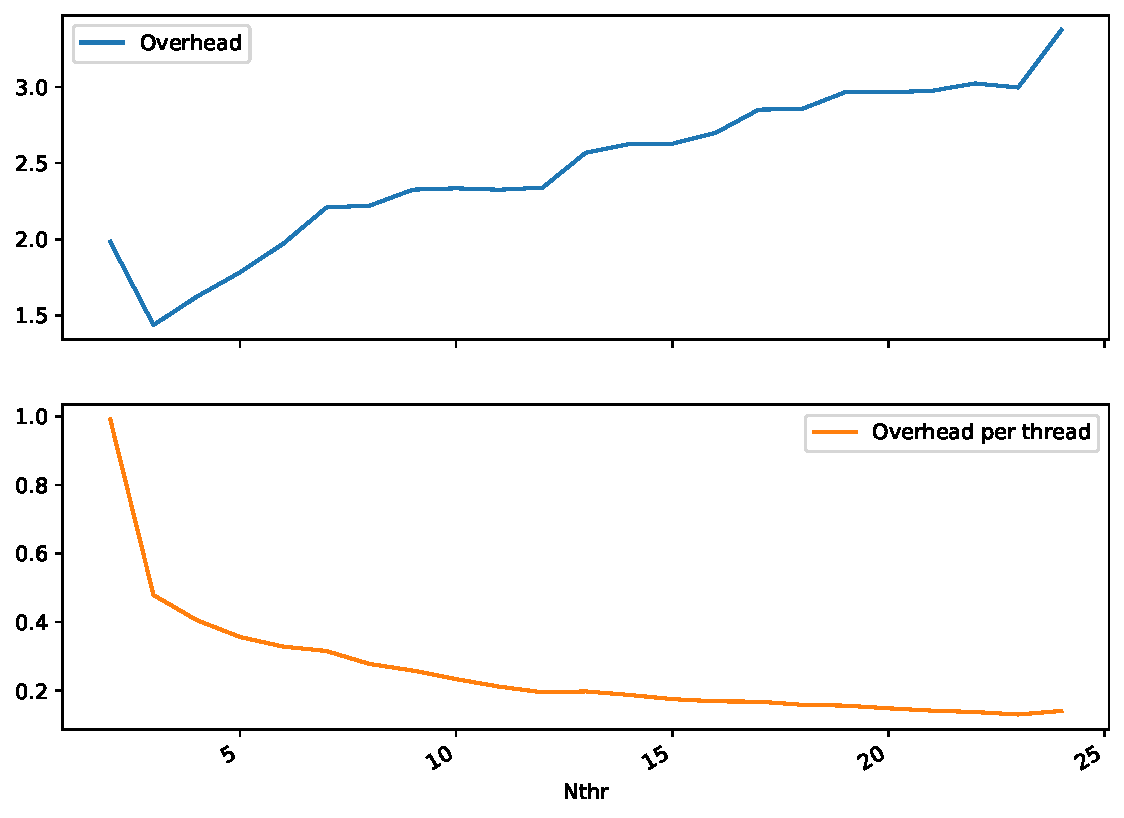
\includegraphics[width=0.9\textwidth]{data/parallel_sub.pdf}
\end{figure}
\null\vfill

\pagebreak
\null\vfill
\subsection{Task creation and synchronization}

Figure~\ref{fig:task} shows the overhead of task creation and synchronization. There is clearly a linear
trend between the number of tasks created and the overhead of the program, which is further reinforced by the
fact that the overhead per task is nearly the same throughout the different number of tasks (the y
axis ranges from 0.122 to 0.130. As with the previous section, the overhead per task is more noticeable
at the very first few values.

\vspace{5em}

\begin{figure}[H]
    \centering
    \caption{Overhead plots for \texttt{pi\_omp\_tasks 10 1}}%
    \label{fig:task}
    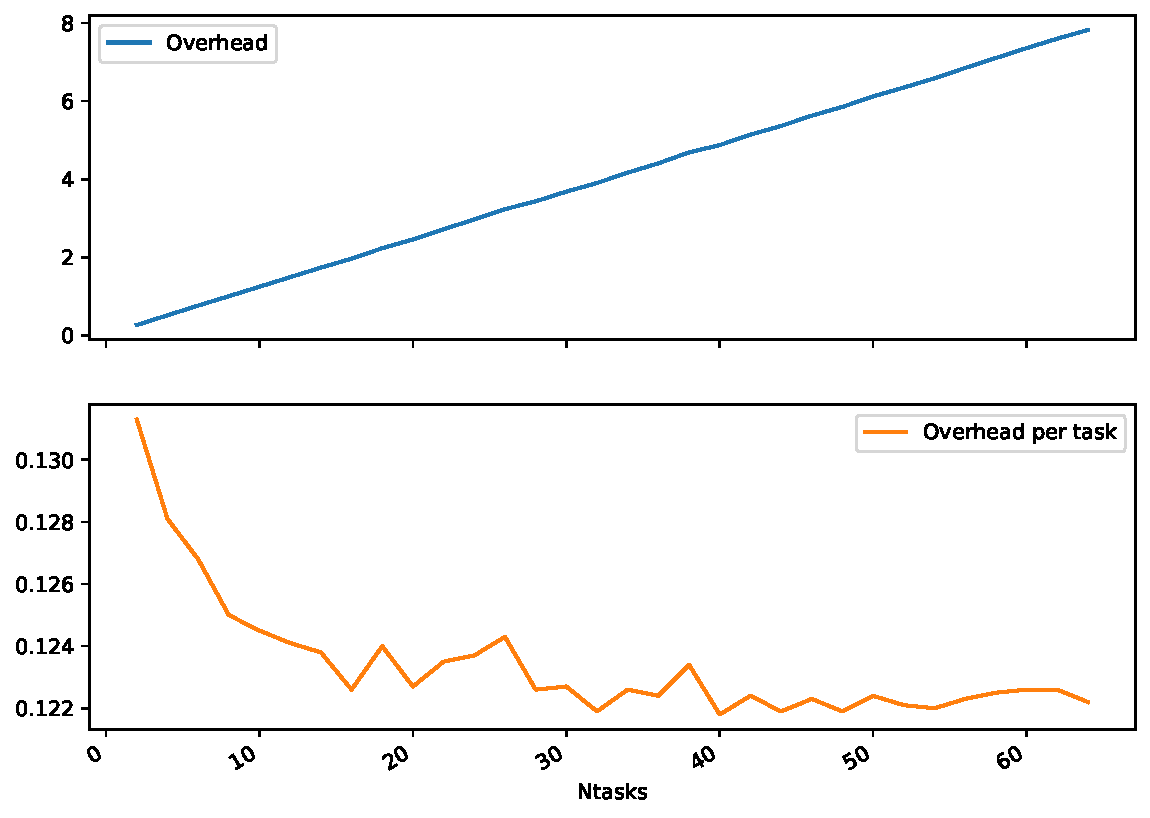
\includegraphics[width=0.9\textwidth]{data/tasks_sub.pdf}
\end{figure}

\null\vfill

\end{document}